In leading order we have to consider photon-gluon-fusion (PGF), that is
\begin{equation}
\Pggx(q) + \Pg(k_1) \rightarrow \PQ(p_1)+\PaQ(p_2)
\end{equation}
with two contributing diagrams depicted in figure \ref{fig:FeynLO}.
\begin{figure}[ht!]
\centering
\begin{subfigure}[t]{.4\textwidth}
	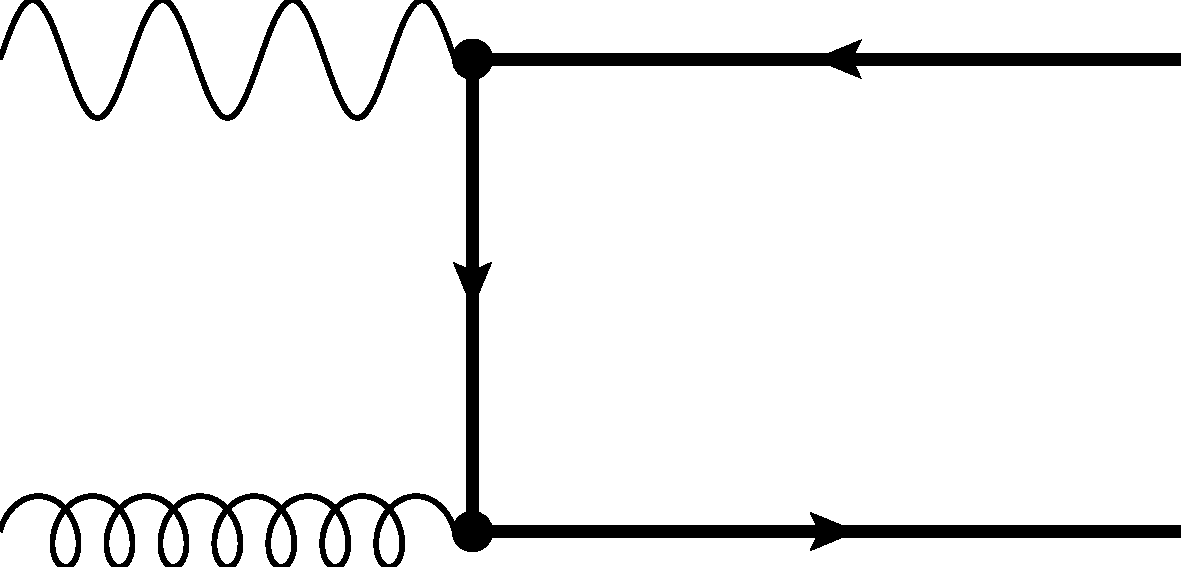
\includegraphics[width=\textwidth]{pyfeyn/lo-1}
	\caption{$i\varepsilon^{\mu}_{\Pgg}(q)\varepsilon^{\nu}_{\Pg}(k_1)\Md^{(0),1}_{\mu\nu}$}
\end{subfigure}\hspace{.15\textwidth}%
\begin{subfigure}[t]{.4\textwidth}
	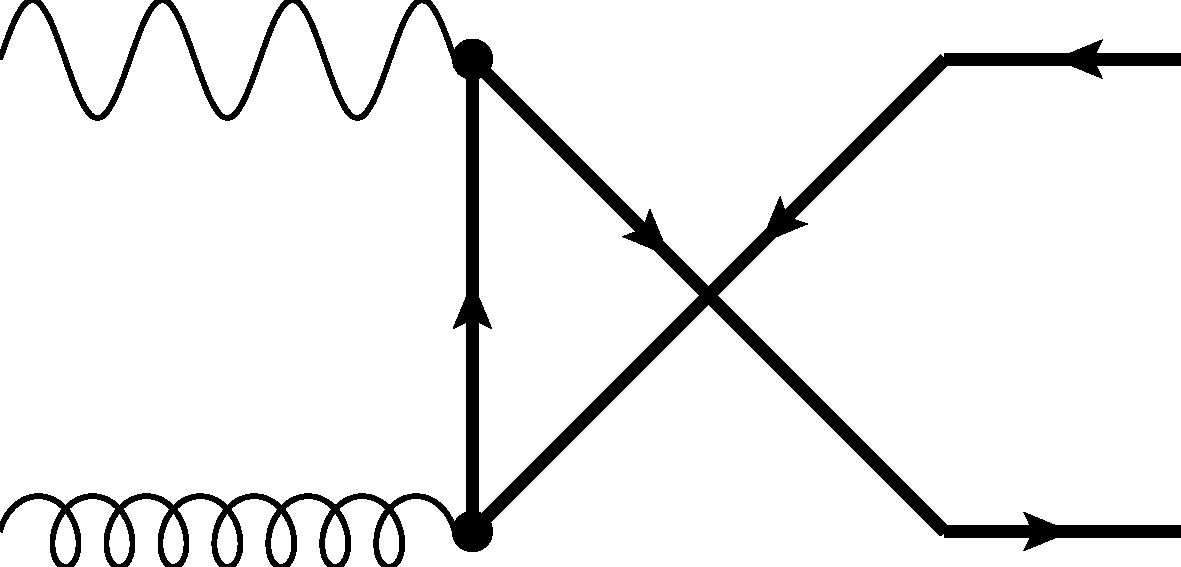
\includegraphics[width=\textwidth]{pyfeyn/lo-2}
	\caption{$i\varepsilon^{\mu}_{\Pgg}(q)\varepsilon^{\nu}_{\Pg}(k_1)\Md^{(0),2}_{\mu\nu}$}
\end{subfigure}
\caption{leading order Feynman diagrams}\label{fig:FeynLO}\fxerror{shift to appendix?}
\end{figure}

The result can then be written as
\begin{equation}
\hat {\mathcal P}_{\vec k}^{\Pgg,\mu\mu'}\hat {\mathcal P}_{\vec k}^{\Pg,\nu\nu'}\sum_{j,j'=1}^2\Md^{(0),j}_{\mu\nu}\left(\Md^{(0),j'}_{\mu'\nu'}\right)^* = 8g^2\mu_D^{-\epsilon}e^2e_H^2 N_C C_F B_{\vec k,QED}
\end{equation}
where $g$ and $e$ are the strong and electromagnetic coupling constants respectively, $\mu_D$ is an arbitray mass parameter introduced to keep the couplings dimensionless and $e_H$ is the magnitude of the heavy quark in units of $e$. Further $N_C$ corresponds to the gauge group $SU(N_C)$ and the color factor $C_F=(N_C^2-1)/(2N_C)$ refers to the second Casimir constant of the fundamental representation for the quarks. We then find:
\begin{align}
B_{\tVV,F_2,\tQED} &= \left[-1 - \frac{6q^2}{s'} - \frac{6q^4}{{s'}^2} + \frac{q^2(6m^2+s) +2m^2 s + {s'}^2/2}{t_1u_1} - \frac{(2m^2+q^2)m^2{s'}^2}{(t_1 u_1)^2} \right] \nonumber\\
 &\hspace{20pt}+\frac{\epsilon}{2}\left[ -1 + \frac{s^2-q^2s'}{t_1u_1} - \frac{m^2q^2{s'}^2}{t_1^2u_1^2} \right] + \epsilon^2\frac{{s'}^2}{8t_1u_1}\\
B_{\tVV,F_L,\tQED} &= -\frac{4q^2}{s'}\left(\frac s {s'} - \frac{m^2s'}{t_1u_1}\right)\\
B_{\tVV,2xg_1,\tQED} &= \left\{1+ \frac{2q^2}{s'} - \frac{s'(2(2m^2+q^2)+s')}{2t_1 u_1} + \frac{m^2{s'}^3}{(t_1u_1)^2}+\epsilon\left(-\frac 1 2 + \frac{{s'}^2}{4t_1u_1}\right)\right\}(1+\epsilon)
\end{align}
\begin{align}
B_{\tAA,F_2,\tQED} &= \frac{{m^2} {s'}^2 (1+\epsilon ) (2+\epsilon ) (12 {m^2} (-1+\epsilon )+{q^2} (-6+(-3+\epsilon ) \epsilon ))}{12 (t_1 u_1)^2}-\nonumber\\
 &\hspace{15pt} \frac{(1+\epsilon ) \left(8 {s'}^3 \epsilon +12 {q^6} (2+\epsilon )+12 {q^4} {s'} (2+\epsilon )+{q^2} {s'}^2 (4+\epsilon  (20-(-3+\epsilon ) \epsilon ))\right)}{4 {q^2} {s'}^2}-\nonumber\\
 &\hspace{15pt}\frac{(1+\epsilon )}{48 {q^2} (t_1 u_1)}\left({q^2} (2+\epsilon ) (-6+(-3+\epsilon ) \epsilon ) \left(4 {q^4}+4 {q^2} {s'}+{s'}^2 (2+\epsilon )\right)\right.\nonumber\\
 &\hspace{40pt} \left. +48 {m^2} \left(-{s'}^2 (-2+\epsilon )+{q^4} (-4+\epsilon ) (2+\epsilon )+{q^2} {s'} \left(-2+\epsilon +\epsilon ^2\right)\right)\right)\\
B_{\tAA,F_2,\tQED} &= -\frac{{m^2} {s'}^2 (1+\epsilon ) (2+\epsilon ) (12 {m^2}+{q^2} \epsilon )}{6 (t_1 u_1)^2}-\nonumber\\
 &\hspace{15pt}\frac{(1+\epsilon ) \left(4 {s'}^3 \epsilon +4 {q^6} (2+\epsilon )+4 {q^4} {s'} (2+\epsilon )+{q^2} {s'}^2 \epsilon  (6+\epsilon )\right)}{2 {q^2} {s'}^2}+\nonumber\\
 &\hspace{15pt}\frac{(1+\epsilon )}{24 {q^2} (t_1 u_1)} \left(24 {m^2} \left({s'}^2 (-2+\epsilon )+4 {q^4} (2+\epsilon )+2 {q^2} {s'} (2+\epsilon )\right)+\right.\nonumber\\
 &\hspace{40pt} \left. {q^2} \epsilon  (2+\epsilon ) \left(4 {q^4}+4 {q^2} {s'}+{s'}^2 (2+\epsilon )\right)\right)\\
B_{\tAA,2xg_1,\tQED} &= \frac{(1+\epsilon)^2(2-\epsilon)}{2}\left[1+\frac{2q^2}{s'}-\frac{2s'(2m^2+q^2)+{s'}^2}{2t_1u_1} + \frac{m^2{s'}^3}{(t_1u_1)^2} \right.\nonumber\\
&\hspace{40pt}\left. + \left(-1+\frac{{s'}^2}{2t_1u_1}\right)\frac{\epsilon}{2}\right]
\end{align}
\begin{align}
B_{\tVA,xF_3,\tQED} &= \frac{s'(1+\epsilon)(2+\epsilon)}{t_1-u_1}\left\{-1-\frac{\epsilon}{2}-2\frac{q^2}{{s'}} - 2\frac{q^4}{{s'}}- \frac{m^2q^2{s'}^2}{2(t_1u_1)^2} \right.\nonumber\\
 &\hspace{40pt}\left. + \frac{4q^2(4m^2+q^2+s')+{s'}^2(2+\epsilon)}{t_1 u_1}\right\}\\
B_{\tVA,g_4,\tQED} &= \frac{s'(1+\epsilon)}{t_1-u_1}\left\{-2+\epsilon - 4\frac{q^2}{s'} - \frac{m^2{s'}^3}{(t_1u_1)^2} + \right.\nonumber\\
 &\hspace{40pt}\left. \frac{s'(16m^2 + 4q^2 + s'(2-\epsilon))}{4 t_1 u_1} \right\}\\
B_{\tVA,g_L,\tQED} &= 0
\end{align}
\begin{align}
B_{\vec k,\tQED} &= B^{(0)}_{\vec k,\tQED} + \epsilon B^{(1)}_{\vec k,\tQED} + \epsilon^2 B^{(2)}_{\vec k,\tQED}
\end{align}

